% $Id: template.tex 11 2007-04-03 22:25:53Z jpeltier $

\documentclass{vgtc}                          % final (conference style)
% \documentclass{acmart}                          % final (conference style)
%\documentclass[review]{vgtc}                 % review
%\documentclass[widereview]{vgtc}             % wide-spaced review
%\documentclass[preprint]{vgtc}               % preprint
%\documentclass[electronic]{vgtc}             % electronic version

%% Uncomment one of the lines above depending on where your paper is
%% in the conference process. ``review'' and ``widereview'' are for review
%% submission, ``preprint'' is for pre-publication, and the final version
%% doesn't use a specific qualifier. Further, ``electronic'' includes
%% hyperreferences for more convenient online viewing.

%% Please use one of the ``review'' options in combination with the
%% assigned online id (see below) ONLY if your paper uses a double blind
%% review process. Some conferences, like IEEE Vis and InfoVis, have NOT
%% in the past.

%% Figures should be in CMYK or Grey scale format, otherwise, colour 
%% shifting may occur during the printing process.

%% These few lines make a distinction between latex and pdflatex calls and they
%% bring in essential packages for graphics and font handling.
%% Note that due to the \DeclareGraphicsExtensions{} call it is no longer necessary
%% to provide the the path and extension of a graphics file:
%% \includegraphics{diamondrule} is completely sufficient.
%%
\ifpdf%                                % if we use pdflatex
  \pdfoutput=1\relax                   % create PDFs from pdfLaTeX
  \pdfcompresslevel=9                  % PDF Compression
  \pdfoptionpdfminorversion=7          % create PDF 1.7
  \ExecuteOptions{pdftex}
  \usepackage{graphicx}                % allow us to embed graphics files
  \DeclareGraphicsExtensions{.pdf,.png,.jpg,.jpeg} % for pdflatex we expect .pdf, .png, or .jpg files
\else%                                 % else we use pure latex
  \ExecuteOptions{dvips}
  \usepackage{graphicx}                % allow us to embed graphics files
  \DeclareGraphicsExtensions{.eps}     % for pure latex we expect eps files
\fi%

%% it is recomended to use ``\autoref{sec:bla}'' instead of ``Fig.~\ref{sec:bla}''
\graphicspath{{figures/}{pictures/}{images/}{./}} % where to search for the images

\usepackage{microtype}                 % use micro-typography (slightly more compact, better to read)
\PassOptionsToPackage{warn}{textcomp}  % to address font issues with \textrightarrow
\usepackage{textcomp}                  % use better special symbols
\usepackage{mathptmx}                  % use matching math font
\usepackage{times}                     % we use Times as the main font
\renewcommand*\ttdefault{txtt}         % a nicer typewriter font
\usepackage{cite}                      % needed to automatically sort the references
\usepackage{tabu}                      % only used for the table example
\usepackage{booktabs}                  % only used for the table example
%% We encourage the use of mathptmx for consistent usage of times font
%% throughout the proceedings. However, if you encounter conflicts
%% with other math-related packages, you may want to disable it.


\usepackage{minted}


%% If you are submitting a paper to a conference for review with a double
%% blind reviewing process, please replace the value ``0'' below with your
%% OnlineID. Otherwise, you may safely leave it at ``0''.
\onlineid{0}

%% declare the category of your paper, only shown in review mode
\vgtccategory{Research}

%% allow for this line if you want the electronic option to work properly
\vgtcinsertpkg

%% In preprint mode you may define your own headline.
%\preprinttext{To appear in an IEEE VGTC sponsored conference.}

%% Paper title.

\title{Avatar Modeling with Inverse Kinematics}

%% This is how authors are specified in the conference style

%% Author and Affiliation (single author).
%%\author{Roy G. Biv\thanks{e-mail: roy.g.biv@aol.com}}
%%\affiliation{\scriptsize Allied Widgets Research}

%% Author and Affiliation (multiple authors with single affiliations).
\author{Alexander Gullickson \thanks{e-mail: gulli173@umn.edu} %
\and Daniel Shervheim\thanks{e-mail: sherv029@umn.edu} }%
%%\and Martha Stewart\thanks{e-mail:martha.stewart@marthastewart.com}}
%%\affiliation{\scriptsize Martha Stewart Enterprises \\ Microsoft Research}

%% Author and Affiliation (multiple authors with multiple affiliations)
% \author{Alexander Gullickson\thanks{e-mail: gulli173@umn.edu}\\ %
%         \scriptsize University of Minnesota - Twin Cities %
% \and Daniel Shervheim\thanks{e-mail: sherv029@umn.edu}\\ %
%      \scriptsize University of Minnesota - Twin Cities }

%% A teaser figure can be included as follows, but is not recommended since
%% the space is now taken up by a full width abstract.
%\teaser{
%  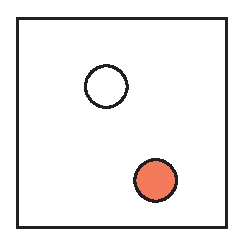
\includegraphics[width=1.5in]{sample.eps}
%  \caption{Lookit! Lookit!}
%}

%% Abstract section.
\abstract{
In this paper, we present a solution for users to embody virtual human avatars in WebXR. The avatar follows the users upper body movements through the use of inverse kinematic solvers. We introduce two avatar controllers based on two different solvers (BoneIK and CCD). We discuss the benefits and drawbacks of each method, as well as the exposed APIs for each method. In supplementary material, we provide our source code and multiple test bed environments.

\\ 
\textbf{Keywords:} Inverse kinematics, avatars, embodiment.
% 
% Citations:
% 1  \cite{simplified} 
% 2  \cite{Analysis} 
% 3  \cite{Distributed}
% 4  \cite{Pose}
% 5  \cite{On} 
% 6  \cite{Bodiless}
% 7  \cite{VR-Replay}
% 8  \cite{Avatar}
% 9  \cite{Influence}
% 10 \cite{First}
% 11 \cite{Application}
% 12 \cite{Real-Time}
% 13 \cite{HumanUpperBody}
% 14 \cite{FastIK}
% 15 \cite{IkTechniques}
% 16 \cite{IkMocap}
% 17 \cite{CCD}
% 18 \cite{FabrikHuman}
% 19 \cite{FabrikOG}

} % end of abstract


%% ACM Computing Classification System (CCS). 
%% See <http://www.acm.org/about/class> for details.
%% We recommend the 2012 system <http://www.acm.org/about/class/class/2012>
%% For the 2012 system use the ``\CCScatTwelve'' which command takes four arguments.
%% The 1998 system <http://www.acm.org/about/class/class/2012> is still possible
%% For the 1998 system use the ``\CCScat'' which command takes four arguments.
%% In both cases the last two arguments (1998) or last three (2012) can be empty.

\CCScatlist{
  \CCScatTwelve{Human-centered computing}{Human computer interaction (HCI)}{Interaction paradigms}{Virtual reality};
  \CCScatTwelve{Computing methodologies}{Computer graphics}{Animation}{Procedural animation}
}

%\CCScatlist{
  %\CCScat{H.5.2}{User Interfaces}{User Interfaces}{Graphical user interfaces (GUI)}{};
  %\CCScat{H.5.m}{Information Interfaces and Presentation}{Miscellaneous}{}{}
%}
% \begin{CCSXML}
% <ccs2012>
%   <concept>
%       <concept_id>10003120.10003121.10003124.10010866</concept_id>
%       <concept_desc>Human-centered computing~Virtual reality</concept_desc>
%       <concept_significance>500</concept_significance>
%       </concept>
%   <concept>
%       <concept_id>10010147.10010371.10010352.10010378</concept_id>
%       <concept_desc>Computing methodologies~Procedural animation</concept_desc>
%       <concept_significance>500</concept_significance>
%       </concept>
%  </ccs2012>
% \end{CCSXML}

% \ccsdesc[500]{Human-centered computing~Virtual reality}
% \ccsdesc[500]{Computing methodologies~Procedural animation}

%% Copyright space is enabled by default as required by guidelines.
%% It is disabled by the 'review' option or via the following command:
% \nocopyrightspace

%%%%%%%%%%%%%%%%%%%%%%%%%%%%%%%%%%%%%%%%%%%%%%%%%%%%%%%%%%%%%%%%
%%%%%%%%%%%%%%%%%%%%%% START OF THE PAPER %%%%%%%%%%%%%%%%%%%%%%
%%%%%%%%%%%%%%%%%%%%%%%%%%%%%%%%%%%%%%%%%%%%%%%%%%%%%%%%%%%%%%%%%

\begin{document}

%% The ``\maketitle'' command must be the first command after the
%% ``\begin{document}'' command. It prepares and prints the title block.

%% the only exception to this rule is the \firstsection command
\firstsection{Introduction and Motivation}

\maketitle
    
    We are not aware of any packages for Babylon.js (our WebXR engine of choice) that allow the user to embody an avatar. We aim to fill that gap. Our package gives users direct control over a virtual human avatar. Our package provides two sample environments with mirrors to test our method. We used inverse kinematics to control the upper body. Due to the lack of lower body sensors, we removed the lower body from the avatar mesh. We attempted various ways to control the lower body through animation blending. Due to restrictions in Babylon, and our own schedule, we decided it was infeasible.
    
    WebXR currently only supports rendering two controller meshes (one for each XR controller). This is fine for many applications and (for the most part) not detrimental to immersion \cite{Bodiless}. Yet there are still some applications where an avatar is essential to the experience. Interacting with others in a virtual world, and studies on empathy in VR, for example.
    
    Our goal is that users will be able to interact with their virtual avatar as if it were an extension of themselves. For example, the avatar should mimic the users motion as close as possible. We believe that this can lead to increased immersion over the default floating controller models.

    Our proposed package expands the possibility for 3D interaction in WebXR. We believe that it will enable the creation of applications that were not possible in Babylon.js. One such example is virtual meetings. A team at Cornell University conducted a study on the effectiveness conducting business meetings in VR \cite{VR-Replay}.  They recorded a significant benefit for users who embodied virtual avatars versus those who did not. Users were both more collaborative and productive. In the age of the COVID-19 pandemic, most meetings of all kinds have shifted to the virtual stage. We believe the virtual avatar model could have a positive effect on people dealing with increased isolation and "Zoom fatigue".
    
    Another interesting use case is industry and design \cite{Distributed}. Automakers in particular are flocking to VR as a creation tool. Two designers could work together on a car model in VR, for example. They could annotate and sculpt the same prototype from thousands of miles apart.
    
    Finally, there are also uses for a package such as ours in game design as well. Embodying a virtual avatar helps increase immersion in the virtual world. These are all examples of possible 3D user interaction use cases for our package.
    
\section{Related Work}

    In this section we present a brief overview of the various studies, algorithms, and processes relevant to our goal.

\subsection{Compelling Avatars}

    Embodiment is the sense that a user actually inhabits the virtual world they are viewing. It is one of the most important factors for immersive VR experiences. There are many factors that can both increase and decrease the embodiment a person feels. In this paper, we will focus only on the illusion of virtual body ownership (IVBO). Lugrin et al. \cite{Avatar} conducted a study to determine the necessary components required to illicit a strong IVBO response. They found that, in general, a generic stylized humanoid avatar was enough to induce a strong response. Interestingly enough, they cautioned against a relentless pursuit of realism. They found that if a realistic avatar was not "realistic enough", it decreased IVBO due to the uncanny valley effect. Their results were further confirmed in additional studies\cite{Influence}.
    
    Crucial to maintaining a strong IVBO is the quality of the virtual avatars pose – especially in how well it mirrors the user. If a person raises their arm, they expect their virtual avatar to do the same. When virtual avatars fail to mirror their users, it often leads to decreased IVBO and even frustration. Realistic and accurate motion is then a key concern in increasing IVBO. This introduces an interesting problem. How does virtual avatar know what pose the user is in? An intuitive solution might be to attach trackers all along the users body and feed those positions into the avatar. Unfortunately this solution is both expensive and complicated to setup. Additionally, most consumer VR hardware has limited support for additional sensor input. For example, the Oculus Quest allows input only from the included 6DOF headset and two 6DOF controllers.

\subsection{Inverse Kinematics}
    
    Before detailing inverse kinematics, we would like to talk briefly about articulated bodies and forward kinematics.

    Both forward and inverse kinematics operate on articulated bodies. An articulated body is a tree structure composed of rigid links connected by joints. Links are rigid lines of a fixed length. Joints can be either revolutionary or prismatic. A prismatic joint allows links to expand and contract along a fixed axis, like a pirate's telescope. Revolutionary joints allow links to rotate along an axis within a range of angles. Additionally, many links can connect to a single joint. There is typically a single "root" link from which all others grow. The terminating links are called "end effectors". Using these primitives, an articulated body can be constructed to represent almost any skeletal form. 
    
    Forward kinematics is the process of determining end effector configurations (position and orientation) from a set of initial joint configurations. A simple algorithm starts at the root link, and recursively applies each joint configuration.

    Inverse kinematics is the opposite problem. Given a set of end effector configurations, inverse kinematics attempts to solve for the set of joint configurations necessary to produce those end effector configurations. This is a complicated problem, with many proposed solutions.
    
\subsection{Applied Inverse Kinematics}
    
    There are many methods to solve the inverse kinematic problem \cite{IkTechniques}. In this section we will detail some of the most common ones.
    
    CCD, or "cyclic coordinate descent" is a common inverse kinematic solver \cite{CCD}. It starts at the end effectors and works up to the root.  For each joint, it computes the rotation that moves the attached link as close as possible to the goal configuration. It is easy to implement but can take many iterations to converge to a solution. Additionally, it can suffer from numerical instabilities. It also only supports one articulated chain by default, although extensions exist to overcome this limitation. Aristidou et al. gives a nice overview of such extensions in section 5.3 of his survey on inverse kinematics algorithms \cite{IkTechniques}. 
    
    FABRIK, or "Forward And Backwards Reaching IK" is another popular solver introduced by Aristidou et al. \cite{FabrikOG}. Rather than solving for angles at each joint from the end effectors to the root, FABRIK traverses the chains backwards and forwards and computes the new joint configurations in position space rather than orientation space \cite{ReviewNewFast}. Like CCD, it still requires multiple iterations to converge to a solution. Because it works in position space rather than orientation space, it tends to exhibit more orientation oscillation over time. In 2015 Aristidou et al. extended their original algorithm to better support humanoid articulated bodies \cite{FabrikHuman}.
    
    Target Triangle \cite{FastIK} is another solution proposed with a number of improvements over traditional CCD. CCD works from the end effectors to the root, which tends to under-value the rotation of the more important joints and over-value the rotation of the less important joints. (For example, when you reach for something, you almost always rotate your shoulder first to get your hand near the object, and then fine-tune your grab by rotating your wrist). Target Triangle works from the root outwards, and produces more natural-looking poses than CCD. Target Triangle is also faster than CCD when CCD requires more than one iteration.
    
    
\subsection{Inverse Kinematics with Animation Blending}
\label{ikwithanim}
    The inverse kinematic techniques discussed so far are valid forms of full-body avatar control  \cite{Analysis, simplified, On}. Unfortunately they would require sensors on the hips and feet to control the lower body as well as the upper body.

     Inverse kinematics with animation blending by Jiang et al. \cite{Real-Time} is a novel approach to full-body avatar control. It was designed with off-the-shelf consumer virtual reality devices in mind. In this method, inverse kinematics is used to control the upper body while animation blending is used to control the lower body. Inverse kinematics is used on the upper body because the user already has sensors at their hands via the controllers. This gives the head and hand end-effectors for the inverse kinematics algorithm.
    
    The user is often more aware of the position of their upper body rather than their lower body. Thus requiring more accurate algorithms for upper body control, like inverse kinematics. In contrast, the lower body motion is only estimated and replicated through animations with a focus on natural motion. With no sensors on the feet, estimation is the best we can do. Jiang et al. estimates the users gait from the swing of their arms and head velocity. Small discrepancies between the real and virtual worlds in the lower body is okay. There are two reasons for this. While in a VR headset, the user cannot see their actual feet. A small difference will not be perceptible as long as the virtual motion is still a natural walking gait. The user also does not typically focus directly on the avatar's feet as they walk. Instead, they generally look where they are going. 
    
    If the user needs to take precise steps like walking on a narrow balance beam, this would not be the right technique to use. Jiang et al. also extended the lower body control with animations like crouching and kneeling.  To do so required a neural network trained on different user motions. Their final implementation took 7ms on average to determine the avatar position each frame. They used an HTC Vive and Intel I5 / Nvidia GTX 980 PC.

   Inverse kinematics with animation blending has many advantages and disadvantages. The primary advantage is the possibility to function with off-the-shelf consumer devices. Additionally, the user does not have to attach sensors to their feet.  Unfortunately, there are some disadvantages. The biggest is that the user does not have direct control over their virtual legs. This method cannot detect any isolated movement of the users physical legs without the arm swinging and head movement. It cannot, for example, capture the action of stepping in place. Also, the avatar will only be able to perform the leg animations it has been fed. Any animation the virtual leg performs must be provided beforehand. With added animations, the neural network would need to be further trained which could possibly lead to more error prone results. Another disadvantage is the possibility of greater latency in the user to avatar movement. The Jiang et al. \cite{Real-Time} solution having a latency of 7 ms was using hardware far superior than the Oculus Quest.
    
\section{Implementation}

    The following lays out our overall implementation and any known problems incurred during the implementation. The are two different IK solvers used and each were implemented with the other in mind. Yet some small differences will exist between them due to both the inherent limitations of the specific solver and the development of each on separate GitHub branches. Known differences will be noted.

\subsection{Test Bed Layout}

    The purpose of the testbed was to evaluate the capabilities of the inverse kinematic methods implemented. As such, we implemented two different testbed environments. One testbed was a basic scene consisting of four mirrors and a ground. The other testbed was a more complex apartment scene with one large mirror. The purpose of the basic testbed was to evaluate how well each inverse kinematic algorithm worked as a stand-alone method. In this testbed, the only latency issues should be a result of updating the limb positions or rendering the mirrors. The purpose of the more apartment testbed is to observe how well the limbs update in a scene more representative of an actual game environment. In both testbeds, mirrors are employed to further evaluate the limb positions beyond just looking down at the avatar. It should be noted that the mirrors are set to the highest resolution possible to make seeing the avatars limb rotation clear in the mirrors. This does require a non-insignificant amount of computing power on the Oculus Quest, but it is deemed a necessary trade off. Additionally, basic teleportation has been added to the testbeds. This allows the user to both navigate the scene and get closer to the mirrors to inspect themselves. Teleportation is triggered by pressing the right thumb stick forward when the controller is pointed at the ground. A halo will show up at the teleportation target position. The teleportation procedure moves the environment and not the user to avoid impacting any of the inverse kinematic solvers or avatar properties which might break the inverse kinematics. Because of this, rotation during teleportation was not implemented.

\subsection{Calibration Procedure}

    The intent of the calibration procedure is to better match the avatar’s body to the user’s proportions. The process is initiated and advanced by pressing the “A-button” on the Oculus Quest’s right controller. If at anytime the user needs to stop the calibration, they are able to press the “B-button” to escape. Currently the CCD IK avatar exposes an onCalibrationStateChanged observable that users can subscribe to in order to change aspects of the scene in response to the new calibration state. For example, we use it to change the animations on the guide avatar. We would eventually like to expose an API for setting the controls that advance or cancel the calibration, but for now that functionality is hard-coded into the A and B buttons. The overall process is straightforward. Once the calibration is initiated, a calibration avatar will appear in the scene with a guiding prompt. The prompt will inform the user a calibration has been initiated and how to advance or cancel the calibration. After advancing the calibration, the calibration avatar will form a T-Pose and request the user to match its pose. After matching the pose, the user will press the “A-Button” again, and the calibration avatar will give a success dance with a prompt informing the calibration process has been complete. At this time, the system will have calculated the user’s height and arm lengths, and then it scales the model appropriately. All the bones are scaled based on the user’s height, and the arm bones are scaled again based on arm span to get the appropriate proportions.

    We experimented with more complicated calibration procedures. We tried having the user bend their arms at 90-degrees as well as touching their shoulders. This would then give the system data about the user’s chest width, upper arm length, and forearm length. In the end, we found that this did not lead to more accurate results. One reason being that more error could be brought in by having the user form an exactly 90-degree angle with their arms while being blindfolded. Instead, average body proportions were used based on the information received from the controller and headset positions. For example, the average chest width is roughly 22\% of the total arm span \cite{openlab}. By using these estimates, we found it made the whole process simpler and lead to results that are perceptually equivalent. 

Overall, the calibration procedure does an effective job of scaling the avatar correctly in a system with no inverse kinematics or when the CCD inverse kinematic algorithm has been applied. The BoneIKController system was only able to scale the user’s height and torso width but not their arm lengths. This is a limitation of the Babylon.js implementation of bone inverse kinematics and was not something we could correct for. The following solutions were attempted. The first attempt was to just scale the arm bones by applying the desired scaling to each bone. It was determined that when the BoneIK positions are updated, a matrix update occurs which resets the bones scaling. The next attempt was to scale the bones to the desired length after the BoneIK update method is called but before the frame is rendered. This would update the scaling on the bones, but the bone positioning was calculated for the default scale bones, so the hands would no longer align with the controller positions. The next attempt was to remove the default calibration and wait to apply the BoneIK to the skeleton until after the calibration had taken place. Again, it was found that the bone IK algorithm would reset the scaling to the default scaling of 1 every time the new bone positioning was determined. The last resort was to attempt to pull out the Babylon.js implementation into our own file and make the necessary changes to allow the skeleton to be scaled. Although, not fully understanding how their implementation worked lead to this being a dead end. In the end, it was decided that this was just a limitation of the Babylon.js implementation, so other tasks were focused on.

\subsection{Body Forward Vector}
\begin{figure}[tb]
 \centering % avoid the use of \begin{center}...\end{center} and use \centering instead (more compact)
%  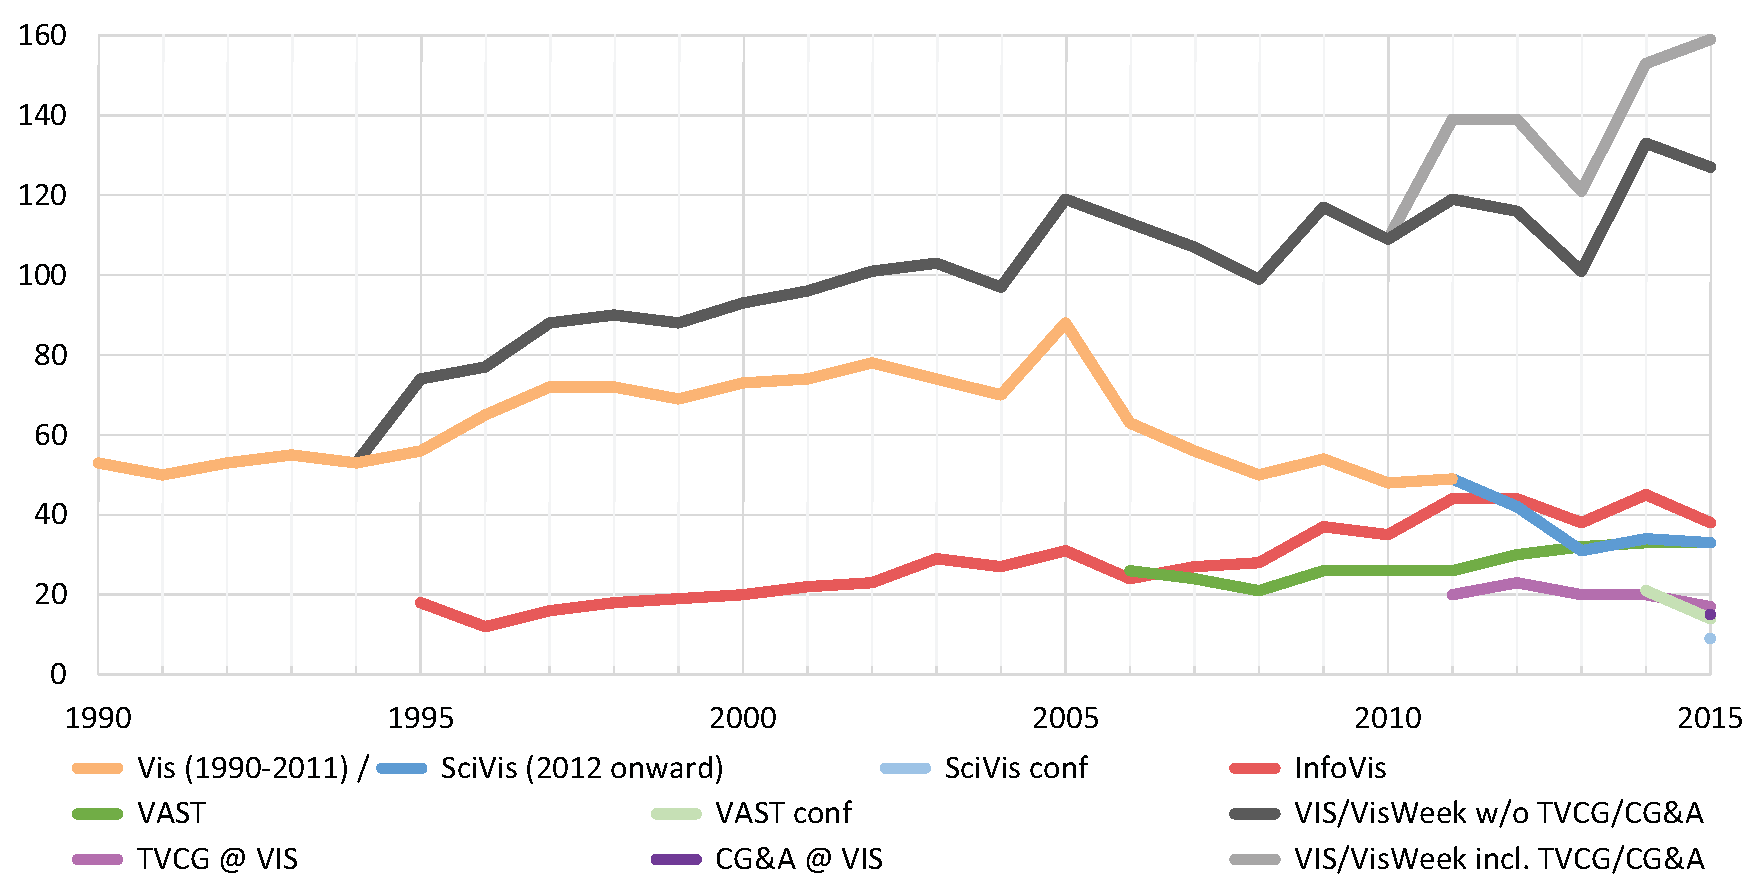
\includegraphics[width=\columnwidth]{paper-count-w-2015-new}
 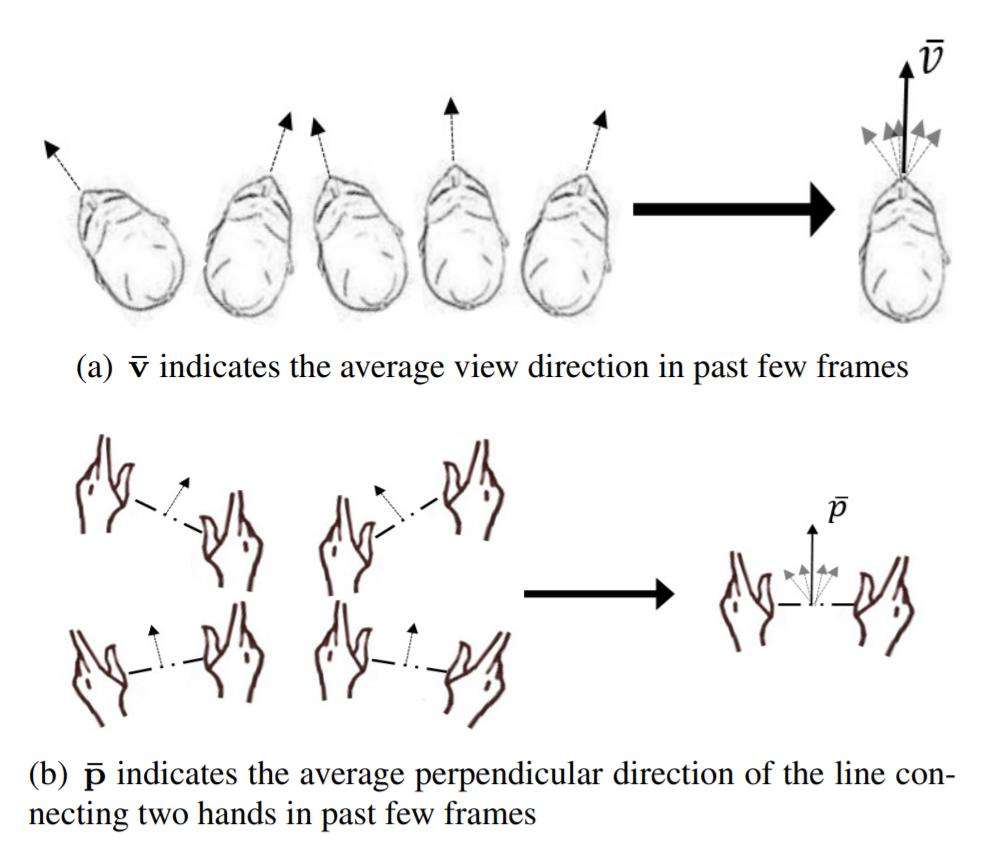
\includegraphics[width=\columnwidth]{pictures/Figure View and controller forward direction.png}
 \caption{ Headset forward vector (a) and controllers forward vector (b) in a pictorial form. The image is from \cite{Real-Time}.}
 \label{fig:forwardVector}
\end{figure}

We quickly realized that the process of determining the body forward vector was an essential task that needed to be completed. The body forward vector is the direction the torso is pointing in the scene. The Oculus Quest has no torso tracker, so this needs to be estimated based on the user’s head orientation and hand positions. The estimation process was adapted from the work of Jiang et al. \cite{Real-Time}. The process begins by averaging the head orientation as well as averaging the hand positions over the last 50 frames. This accounts for any fluctuations from the head or hands moving. If the most recent measurements are not within a small threshold of the average, there values are marked as unstable for the forthcoming calculations. Next, the forward vector of the controllers needs to be determined to reference against the headset orientation forward vector. A depiction of the headset and controller forward vectors are shown in \autoref{fig:forwardVector}. The controller forward vector is found by taking the cross product of the line between the controllers and the unit vector pointing down. The resulting vector is normalized and is the vector perpendicular to the line between the controllers. In addition to these vectors, two angles (aCross and aLinear) are needed to determine the body forward vector (see \autoref{fig:aCrossALinearAng}). The first angle, referred to as aCross, is the angle between the headset forward vector and the line going between the controllers. When both the headset and the controllers are stable, this value should be near 90-degrees. An example of this is shown in \autoref{fig:aCrossALinearEx}. The other angle, referred to as aLinear, is the angle going from the headset to the left controller and the line between the controllers. If both the headset and controllers are stable, this value should be near 0-degrees. An example of this is shown in \autoref{fig:aCrossALinearEx}. With the above information, the body forward vector can be determined. There are three main cases to determine the body forward vector. 

\begin{figure}[tb]
 \centering % avoid the use of \begin{center}...\end{center} and use \centering instead (more compact)
%  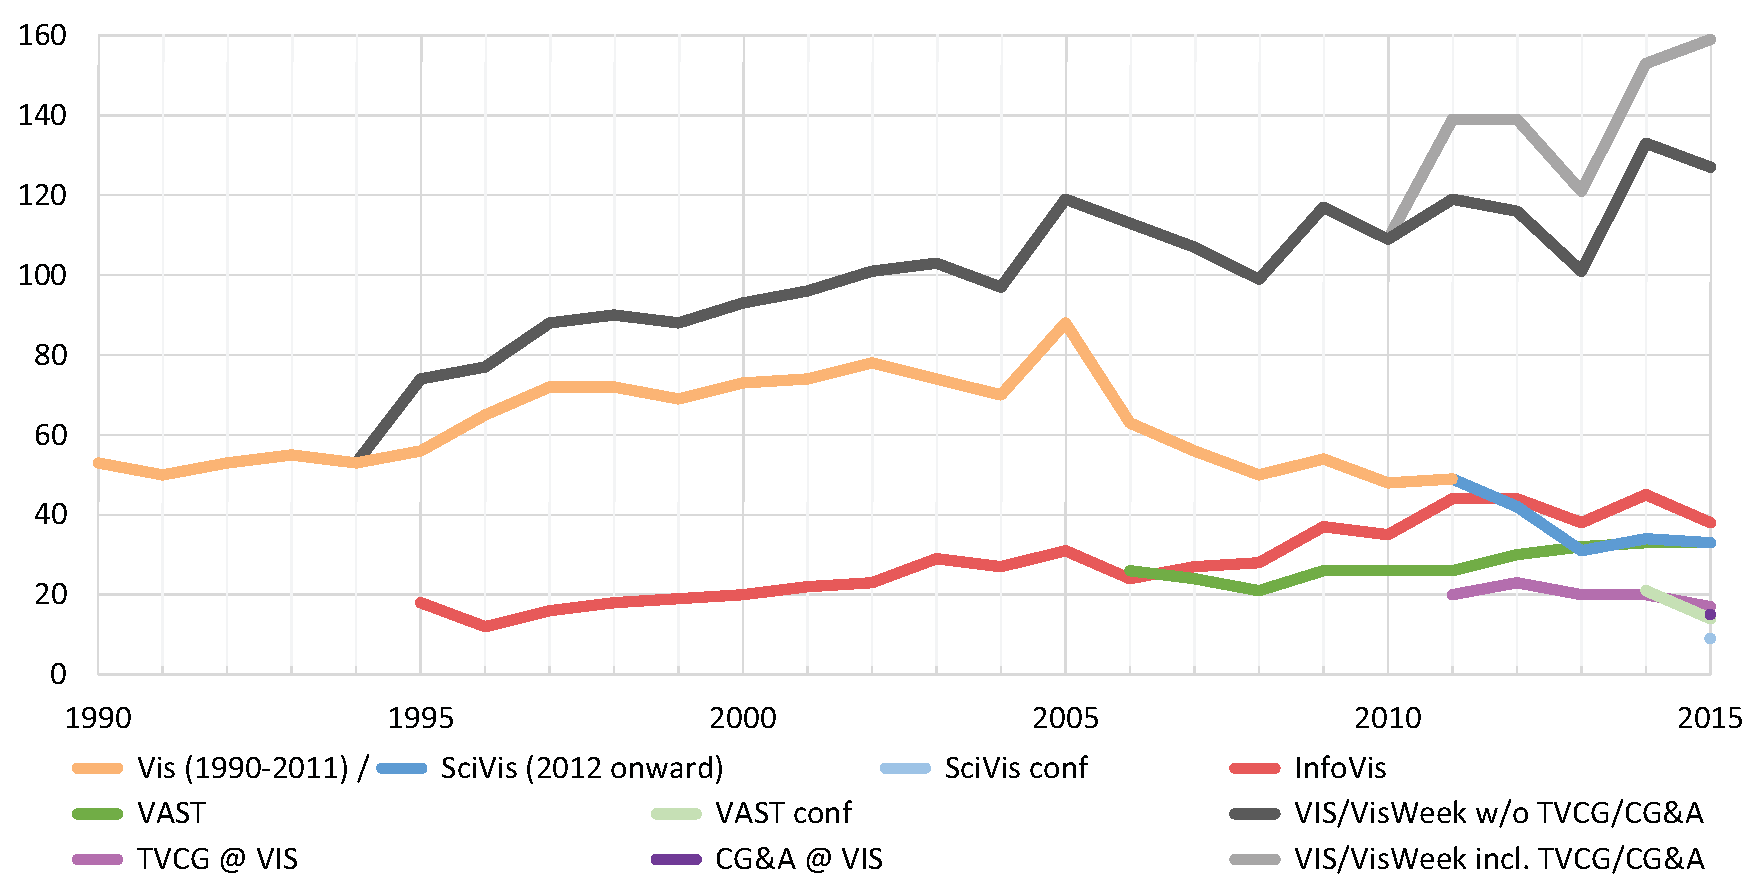
\includegraphics[width=\columnwidth]{paper-count-w-2015-new}
 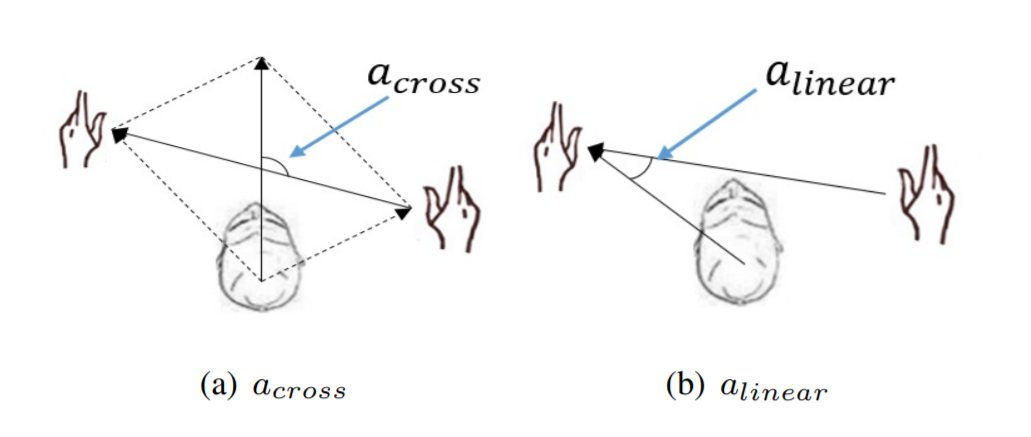
\includegraphics[width=\columnwidth]{pictures/Figure aCross,aLinear.png}
 \caption{A visualization of the aCross (a) and Alinear (b) angles. The image is from \cite{Real-Time}.}
 \label{fig:aCrossALinearAng}
\end{figure}
\begin{figure}[tb]
 \centering % avoid the use of \begin{center}...\end{center} and use \centering instead (more compact)
%  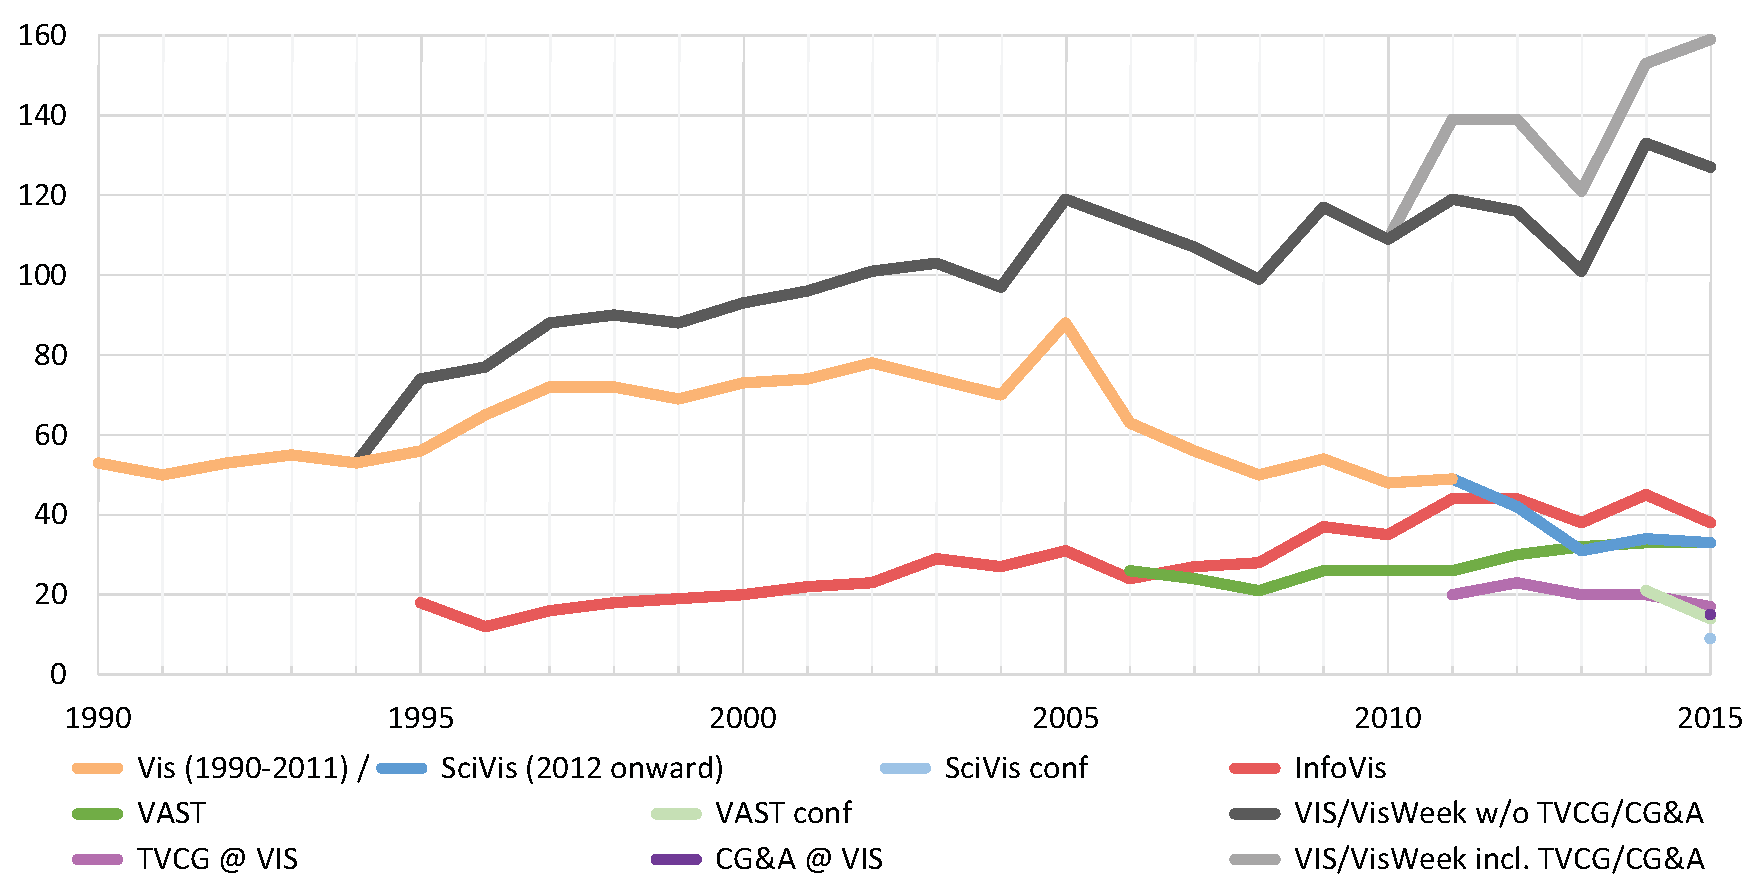
\includegraphics[width=\columnwidth]{paper-count-w-2015-new}
 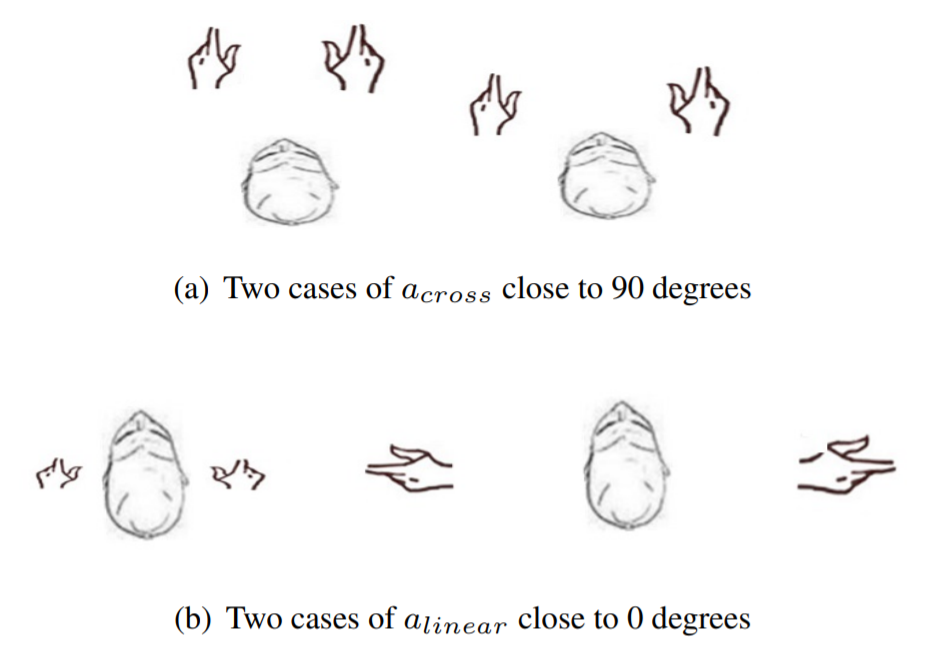
\includegraphics[width=\columnwidth]{pictures/Figure aCross,aLinear valid.png}
 \caption{A visualization of example cases when aCross is near 90-degrees (a) and when aLinear is near 0-degrees (b). The image is from \cite{Real-Time}.}
 \label{fig:aCrossALinearEx}
\end{figure}

The first case is the headset is not stable. In this implementation, the headset is treated as the most important component. If it is not stable, the forward vector cannot be determined, and the torso orientation is not updated. 

The second case is the headset is stable, but the controllers are not stable. This requires a further evaluation to check if the average controller forward vector is roughly the same as the headset forward vector. In the event it is, the body forward vector is set to the headset forward vector. In the event it is not, the body forward vector is set to a blending of the headset and controller forward vectors. 

The final case is both the headset and controllers are stable. An additional check then takes place which checks the aCross angle is near 90-degrees or the aLinear angle is near 0-degrees. Additionally, the controller and headset forward vectors are checked to see if they are roughly the same. If all these checks pass, the body forward vector is set to the headset forward vector. Otherwise, the body forward vector is not updated. 

Finally, the forward vector actually applied to the skeleton will be blend of the previous forward vector with the current reported vector. The blending equation is: 
\begin{equation}
applied Vector = previous Vector * (0.9) + current Vector * (0.1)
\end{equation}

The application of this body forward vector resulted in accurate avatar torso rotation results. When rotating quickly, the torso will sometimes have skipping or delayed rotation, but this occurs only minimally. In the primary application of it, these errors do not occur. Most importantly, it allows the user to look around with the torso remaining static, and it allows the user to move their arms in various motions without effecting the torso rotation.  

It should be noted that the above algorithm was only implemented for the BoneIKAvatar. For the CCDAvatar, we opted for a simpler equation. We use a spherical interpolation between the rotation of the XR headset, and the rotation of the vector perpendicular to the plane formed by the two controllers and the world up vector. We found this provides a fairly accurate forward vector estimation, although it is not as robust as the version employed in the BoneIKAvatar due to not taking the previous history into account.

\subsection{BoneIKController}

The initial inverse kinematics algorithm tested was the use of the BoneIKController. The BoneIKController is a basic two bone IK solver provided by Babylon.js. The solver itself is modeled after Blender’s BoneIK solver. The invocation of the BoneIKController requires the mesh the IK is being applied, the bone at the end effector, a target mesh, and a pole target. The position of the target mesh is the end effector or where the arm will reach for. The pole target is a mesh whose position determines the elbow orientation. After the BoneIKController is initialized, the instance is put in a render loop to always update to the new position before the frame is rendered.

The BoneIKController was utilized in the following manner on each arm. As the limit is on two bones, our implementation is mapped to the forearm and upper arm. This does mean the wrist is the location the solver will try to match and not the hand, but our base testing found this not to be too distracting. The target mesh is a hidden sphere that is parented to the controller. The wrist location will then try and reach for the controller position. Next, the pole position was experimented with. The initial design parented it to the user avatar in a single pole position for both controllers. It was determined, in this design, that the arms could match some poses fairly accurately, but other poses were very error prone. The hand rotation was also skewed on the right hand, so the thumb would be pointed down instead of up. Further research was performed to determine if an algorithm could be applied that would map the pole position to a bone to ensure a more accurate arm orientation the majority of the time. Nothing was readily available, so our own implementation was developed.
 
It was apparent that setting the pole position slightly above and in front of the avatar gave more accurate arm orientations when the hands were further away from the user. On the other hand, a pole position in front of and below the user led to reasonable elbow angles when the hands were near the user. Consequently, a macro and micro pole position was defined for each arm when they were in these two zones. A mesh box was then defined around the avatar with the left and right panels just past the avatars shoulder. The top, bottom, front, and back were far enough away such that the user would not be able to reach them from the center. The pole positions would then flip to either the macro pole or the micro pole depending on whether the target mesh intersected the box around the user. The pole positions and the box were then attached to the avatar’s skeleton, so that it would follow the user as their torso rotated. In testing this method, reasonable elbow positioning results were achieved for the majority of user arm movements, so it was kept as the way pole position was determined. There is a noticeable arm rotation when the arms cross the threshold of the box, but it is a minor one of a couple of degrees and not a large 90- or 180-degree flip. The avatar now has arms that will follow the controllers and the elbows will bend in the correct direction the majority of the time. 

The only other issue that needed solving was the right arm was flipped 90-degrees such that when the thumb should be pointing up, it is actually pointing to the side. This was remedied by resetting the hand rotation by 90-degrees in the y-direction. It should be noted that this does not fix the right arms mesh from being miss rotated. Although, the avatar in use can get away with the rotation error as the mesh is not connected at the joints, and the mesh itself does not have overly defining qualities of which end is which. This completed the main implementation portion of the BoneIKController. There were still a couple of additional things added to the BoneIKController implementation worth mentioning.

The BoneIKController algorithm only moved the user’s hand to the correct position, but it did not handle the correct hand rotation. It was found the controllers rotation axes did not match the hand bone rotation axes exactly, so they needed be remapped to one another. After remapping the axes, hand rotation worked reasonably well when the avatars forearms are pointed straight outwards in the z-axis direction, when the forearm angle deviated, the accuracy went down noticeably. To remedy this, the users hand rotation is only calculated when the hands are between the shoulders, and the pole position is in the micro position. This is deemed an acceptable trade off as in most use cases user hand rotation will occur when the hands are in front of the user and less so when they are away from the user. When the user’s hands are in-front of the user, they are at least somewhat positioned in the z-axis direction. Additionally, the errant hand position at distances away from the user was more distracting than any benefit from allowing rotation. For example, in the T-Pose with the thumbs up, the avatar would think the controllers yaw is at 90-degrees, so the hand would be point straight back. As a result of not being able to control the hands perfectly, hand rotation was only implemented for BoneIKController. It was left in to show the work was performed in getting it to work somewhat, but more time would need to be spent on enhancing it before it would be ready for a mainstream product. 

The BoneIK implementation allows for avatar movement and head rotation. An avatar that is confined to the user standing in one place would not lead to an immersive experience, so additional work was put into allowing the avatar to move with the user. Before every frame is rendered, the avatar’s position is mapped to the headset position. It was discovered in doing so that looking down would lead to the body moving forward because the headset would be in a new position. A number of different approaches were attempted at resolving this with a single one decided on. One approach was to require the user to move past a threshold to update the position. This worked but it led to it being possible to step outside of the avatar if only a small change in movement forwards or backwards was needed. Another solution was to use trigonometry. The avatar’s neck and head would form the hypotenuse of the triangle and taking the length between the neck and head multiplied by the arcsine of the angle the head rotated along an axis would give the displacement along the axis. This displacement could then be subtracted from the user’s position to get the correct position. This had positive results when the user was standing in the default position and looked down or rolled their head to a side. Although, it failed miserably when the user’s torso was rotated at a different angle. In this case, it would displace the body in the incorrect direction. The final approach was much simpler. It simply would always shift the user’s body backwards a small amount when updating the position. When the user looks down, they body can still shift forwards a small amount, but it will still look like the user is just looking down at their chest. This approach does come with a small flaw. The avatar is shifted back a small amount, so now if the user attempts reach directly behind then the hand may show up inside the avatar. In general, the user would not be making motions behind them. If the application this was going into required this behavior, the algorithm would need to be modified to allow for this behavior. In addition to updating the avatars position, the avatars head rotation matches the users head rotation. The axes mapping did need to be adjusted. The pitch was the same between the avatars head and the headset rotation. The yaw needed to be inverted and so did the roll. The last thing that needed to occur was the headset needed to account for the body rotation as the user rotates. This was accomplished by adding the forward vector found earlier to the head’s yaw position. After these corrections were made, the head orientation is mapped exactly between the user and the avatar. 

Overall, our setup for the BoneIKController is able to closely match the user’s arm and head rotation. It is not perfect, but the errors are reasonable given the number of sensors. There are a couple of cautionary points found while implementing. These are mostly the result of Babylon.js providing only a basic IK solver. The first issue was the bones are not able to be re-scaled if the BoneIKController is going to be applied to them. This eliminates the possibility of being able to fully calibrate the avatar to the user. Another aspect discovered while implementing is GLB or GLTF mesh files are not supported. This is due to the fact that when they are imported their skeleton bones are based on transform nodes. In order to update a skeleton bone, the equivalent transform node needs to be found, and then the transform node is updated not the bone. It is possible to get each bone used in the IK process right after it has been updated and apply the rotation and position to the equivalent transform node; however, this needs to be done by the developer as Babylon.js will not do the computation automatically. This process also needs to be done before every frame otherwise the bones will reset to their previous positions. Our implementation did need to make a couple of generalizations to support most use cases at the hindrance of some use cases. The main generalizations are only supporting hand rotation between the shoulders, re-positioning the elbows when the hands cross the shoulder threshold, and positioning the headset to be slightly in front of the body.  In certain situations this may not be the desired behaviour, but our goal was to support most functionality and not all functionality. 

\subsection{CCD IK}

    We also implemented a controller based on a CCD inverse kinematic solver, adapted from Zalo's implementation \cite{Zalo}. Our goal with this version was to investigate whether we could improve upon Babylon's built in BoneIK solver. 

    Our CCD controller maintains an internal skeleton consisting of an array of TransformNodes representing the head, neck, shoulders, elbows, and wrists. The "skeleton" is setup similar to a mesh skeleton (for example, the elbow is a parent of the wrist, and the shoulder is a parent of the elbow). This internal skeleton is purely non-visual, and not inherently connected  to any user avatar mesh.

    Every frame, we compute a new forward vector to drive the yaw rotation of the skeleton. We initially tried using the cross product of the world up vector and the vector between the controllers. We found this provided a reasonable estimate of the users forward direction, with the exception of when the user crossed their arms. This would cause the estimated forward vector to flip 180 degrees. To fix this, we also compute a rotation based on the XR camera forward vector, and then spherically interpolate between them based on the amount that the users arms are crossed (measured by the signed deltaPosition.x between the controllers relative to the XR camera). It is not as sophisticated as the forward vector calculation in the BoneIK controller, but we found it provides a reasonable approximation most of the time. 

    We also update the arms each frame. The left and right arms both consist of a transform chain like so: (shoulder-(elbow-(wrist))). We pass each chain independently into our CCD IK solver, as well as the corresponding left and right controller positions. Our solver attempts to rotate the wrist, elbow, and shoulder such that the wrist bone is as close as possible to the controller position, while maintaining the current shoulder position. Unfortunately we ran into nasty issues with numerical stability over time, so rather than using the outright angles computed by our IK solver, we applied damping based on the delta time to smoothly reach the desired rotation over many frames. This helped prevent the arm chains from exploding, but also overly smoothed the motion to a "floaty" appearance.

    Finally, we use the same head and neck algorithm from the BoneIK controller in order to rotate the skeletons neck joint towards the XR camera look direction.

    All of these algorithms run on the internal skeleton, which is purely non-visual. The final step is to mirror the state of the internal skeleton to the skeleton of the provided user avatar mesh. In general, this is as simple as stepping through the user avatar mesh's skeletal hierarchy and copying the appropriate joint rotations from our internal skeleton. In practice, we found that due to different resting joint orientations we had to offset our internal skeleton rotations in some situations. This is unfortunately unavoidable due to the lack of standards in humanoid skeletal rigging.

    In the end, we found that the CCD controller provided almost equivalent motion to that of the BoneIK controller. We did not implement wrist rotation, but we believe it would not be too difficult given a bit more time.

    That said, our CCD controller does exhibit limitations inherent to the CCD inverse kinematic solver (some of which are unavoidable, and found in any CCD-based solver). The most noticeable is that CCD, by necessity, operates from the end of the kinematic chain to the root. In practice, that means we compute the rotation for the wrist, then the elbow, then the shoulder. This tends to place the strongest changes in rotation on the wrist and elbow, which is completely opposite to how a human typically moves their arms. Usually, we rotate our shoulders a lot to get our wrist in the region of the object we are trying to interact with, and then rotate our wrist a tiny bit for fine-grained control. Due to this backwards solving scheme, the motion produced by our CCD solver can sometimes appear unnatural. The elbow might bend opposite to the way it should, for example. Some of these problems can be mitigated by imposing angle restrictions on the joints, but this is an additional layer of complexity and overhead that we chose not to implement initially.

\subsection{Exposed API}

    In this section we will briefly discuss the API for setting up our controllers. Due to code-base divergence during programming, the process differs slightly between the BoneIK and CCD versions. Eventually we would like to clean these up and unify them under a single interface, but for now we will briefly discuss the setup process for both.

\subsubsection{BoneIK API}

The first step to using our controller is instantiating an instance of our controller class. You can do this easily by calling the constructor. It takes as its only argument a Babylon scene object.
    
\begin{minted}{typescript}
BoneIKAvatar(scene: Babylon.Scene);
\end{minted}

In order to track the XR headset and controllers, you must also register an XR experience object with our controller. This is typically done asynchronously during the scene setup.

\begin{minted}{typescript}
BoneIKAvatar.registerXRExperience(
    xrExperience: Babylon.WebXRDefaultExperience
): void;
\end{minted}

You must also register a calibration guide avatar. This is done with the following method, which takes a MeshAssetTask as its argument. It also takes a BoneDictionary, which is essentially a helper class containing a string dictionary of all of the bone names needed by our controller. It also takes a CalibrationAnimationDictionary, which is a helper class containing a string dictionary of all of the animations needed by our controller. The method will scan the mesh and skeleton in the provided MeshAssetTask, and throw an error if one of the required bones or animations in the dictionary is not found in the skeleton. Finally, it also takes an initial position, rotation, and scale for the guide avatar.

\begin{minted}{typescript}
BoneIKAvatar.registerCalibrationAvatarFromMeshTask(
    task: MeshAssetTask,
    bones: BoneDictionary,
    animations: CalibrationAnimationDictionary,
    position: Vector3,
    rotation: Vector3,
    scale: Vector3
): void;
\end{minted}
    
Similarly, you must also register the user avatar. This is done with the following method, which also takes a MeshAssetTask and a BoneDictionary. Because the user avatar will be driven by our IK controller rather than animations, we do not require a CalibrationAnimationDictionary. We also allow the user to provide initial position, rotation, and scale for the user avatar. Like the guide avatar, this method parses the skeleton in the provided MeshAssetTask and throws an error if one of the bones in the BoneDictionary is not found.

\begin{minted}{typescript}
BoneIKAvatar.registerUserAvatarFromMeshTask(
    task: MeshAssetTask,
    bones: BoneDictionary,
    position: Vector3,
    rotation: Vector3,
    scale: Vector3
): void;
\end{minted}

Finally, the controller must be updated before each render frame.

\begin{minted}{typescript}
BoneIKAvatar.update();
\end{minted}
    
\subsubsection{CCD API}

Please see the \verb|basicScene_CCD.ts| file in the accompanying code \cite{ourcode} for the most minimal example of getting up and running with our CCD-based controller.

Due to divergences in the code path, the setup process for the CCDIKAvatar is slightly different from the BoneIKAvatar, although both enable roughly the same functionality.

The first step to using our CCDIKAvatar is instantiating an instance of the CCDIKavatar class. You can do this with its constructor, which takes a Babylon scene object and a DefaultXRExperience object.

\begin{minted}{typescript}
CCDIKAvatar(
    scene: Babylon.Scene,
    xrExperience: Babylon.WebXRDefaultExperience
);
\end{minted}

The only other required step is to bind a user avatar mesh. You can do this with the following method. It takes the root transform of the user avatar mesh, the skeleton of the user avatar mesh, and a SkeletonBones object. This serves the same purpose as the BoneDictionary in the BoneIKAvatar.

\begin{minted}{typescript}
CCDIKAvatar.bindSkeletalMesh(
    playerMeshRoot: Babylon.TransformNode,
    playerSkeleton: Babylon.Skeleton,
    bones: SkeletonBones
);
\end{minted}

Unlike the BoneIKAvatar, the CCDIKAvatar does not have any built in support for a guide avatar or tutorial process (although it does follow the same A and B pattern to advance the calibration procedure as the BoneIKAvatar). Instead, it exposes an observable that returns the current CalibrationState whenever the calibration state changes. For example, we use it to change the guide avatar animation, and change the visible tutorial text mesh.

\begin{minted}{typescript}
CCDIKAvatar.onCalibrationStateChange.add(
(state: CalibrationState) =>
{
    // Do something based on "state" variable.
});
\end{minted}

Finally, the controller must be updated before each render frame. Unlike the BoneIKAvatars update method, this version requires the time since the last render frame as an argument. This is to apply frame-rate independent damping to the CCD solver.

\begin{minted}{typescript}
CCDIKAvatar.update(deltaTime: number);
\end{minted}

\section{Not Implemented}

\subsection{Lower Body Control}

    We initially planned on implementing lower body control. An example of how to implement it is discussed in section \ref{ikwithanim}. In the end, user avatar walking with animation blending was not implemented. This was initially proposed as a stretch goal, but it never came to fruition for a multitude of reasons. The first being Babylon.js does not natively support skeleton animations when the bones are scaled after the animations are applied. This would mean that the calibration procedure would need to be abandoned. It could possibly be implemented by hacking together the rendering process, but to the best of our abilities, we could not find a way to implement this in a reasonable amount of time. The second reason being a space limitation. In our own real world testing space (2 meters x 2 meters), there would not be enough room to reliably detect users arm swinging. In this amount of space, we could take about 3 steps before reaching the end. Going along with the second point, walking is not the ideal navigation technique for small user spaces which means additional navigation techniques are required. It could potentially be used to enhance the effects of redirected walking or other more advanced navigation techniques, but these techniques would likely need to be developed in conjunction with animated walking to function correctly. Additionally, the user is generally not looking at their feet when walking unless they are being careful where they are stepping. In which case, the animated walking was not going to be stepping in the correct place anyways. Ultimately, it was decided based on the reasoning above to abandon the idea early to allow more time to further develop our two inverse kinematics methods being implemented. To prevent distractions from the legs not moving as the user walks or turns, the legs were removed from the user’s avatar. Also, this allows the user to be either standing or sitting without having their legs in the ground. A basic teleportation mechanism was added to aid in navigating around the scene as well, described in the Testbed Implementation section. 

\subsection{Other IK Algorithms}

    We experimented briefly with other inverse kinematic solvers. We tried both FABRIK by Aristidou et. al. \cite{FabrikOG} and Target Triangle by Song et. al. \cite{FastIK}. We weren't able to get FABRIK working. We did manage to get a Target Triangle solver working, but the motion itself was far worse than our CCD solver. We suspect this is due to some programmer error, but in the end our CCD solver ended up being good enough for our needs so other solvers were not extensively tested beyond our initial attempts.

\section{Discussion}

    The discussion section will go over our personal thoughts about using the virtual avatar. These are not meant to represent scientific data merely our own evaluation of the systems. Items considered include differences between the two IK solvers as well as does the system result in an enhanced immersive experience.

\subsection{BoneIK vs CCD}
    
    The BoneIK and CCD systems can be evaluated based on a multitude of different factors. The first factor considered is how well the IK solver is able to match the correct arm orientation and position. In both cases, the hands are able to orient themselves to the correct position, but the elbows are not always in the correct orientation. The BoneIK system bases this orientation off of the pole vector locations. In doing so, the elbow rotation will always be predetermined based on where the target and pole meshes are at. This allows for impossible bending of the arms to be avoided at the cost of not always having the perfect orientation. On the other hand, the CCD solver uses blending of the current location with the previous locations to determine the next orientation. This allows for almost any orientation to be matched as long as the user is not moving in rapid motions. The downside to CCD is that it allows for impossible rotations to be made. The elbow will continue to rotate past the possible rotation limit to reach the correct position. To remedy this, the avatar mesh selected for CCD does not have distinctive sides to the arms, and the joints are disconnected. In doing so, when the impossible orientations are made, it does not distract the user from the realism of the model. Another consideration in comparing the models is the latency of updating the arm positions. In both implementations, the update is performed before every frame is rendered. Therefore, latency is most noticeable by the frame rate dropping. In both cases, the latency does not appear to be overly apparent when in the basic scene. Latency through frame rate drop is apparent in the large studio scene. This is more an artifact of a high-quality scene being rendered and then mirrored as opposed to the IK solvers. The BoneIK solver will appear to reach the stable positions faster because it does not consider prior values. On the other hand, the CCD solver does take more time to reach the final position due to it using both the current and previous values. 

    The solvers also have small difference in the features implemented between them. The difference in features come from fundamental differences in how the solvers are implemented which make some tasks straight forward in one implementation and complex or even impossible to implement with the other implementation. The most notable case for this is the calibration procedure. It currently is only fully supported with the CCD solver where it will scale to the avatar’s height and arm lengths. The BoneIK version will only scale the height and torso but not the arm lengths. In contrast, the BoneIK solver has a more polished rest of the avatar implementation. This includes the body forward vector updating as described in the Body Forward Vector section; basic hand rotation mapped to the controller’s rotation; and the ability to follow the user in 3-Dimensional space. The CCD solver does attempt to implement some of the functionality described. The body forward vector is implemented based on the average value of the headset and controllers’ positions. This works okay, but it does lead to incorrect torso rotation in certain arm positions. Position tracking in 2-Dimensional space was implemented, but it cannot track the users y-position for the reasons described in the CCD Section.

    In the end, it comes down to which IK solver is the better one to use. This ultimately depends on the specific use case. The BoneIK solver is recommended if the desire is for quick motions or the occasional incorrect arm orientation is okay. If a more precise arm orientation is needed at the cost of being slower to update, the CCD solver is recommended. 

\subsection{Enhanced Immersive Experience}

    At the end of the day, the question to ask is whether or not adding the avatar leads to an enhanced user experience. If the user experience is not enhanced, the IK solvers are just taking computing resources without providing any benefit.  One consideration being does the system illicit an increased IVBO response? In our experience, the majority of the time it does not. Instead, it feels more like controlling a robot than controlling yourself in virtual space. In part, this is due to some bugs in the implementation and lack of capability of the system. The system does not have the sensors to know the exact orientation of either the torso or the elbows. This leads to it making educated guesses which most of the times are correct; however, the couple of times it is incorrect can quickly remove the illusion previously built-up. Another potential reason for this is the avatar itself is very much a non-human. By changing the avatar to a human mesh, it is likely to make it feel more realistic. Although, both implementations work correctly for the raw skeleton, but the meshes can be rotated around the bone incorrectly for example the bicep would be where the triceps should be. Correcting for this in one scenario led to it being incorrect in another. Therefore, the current mesh was used to allow for the incorrect orientation to be less noticeable. 

    Another factor in the IVBO response not being as strong is from the testbed design. The testbeds are good testbeds to test the quality of the IK systems because they allow for the bone positions and rate of update to be observed in two different environments. However, the testbeds lack situations where having an avatar is overly useful. An example better testbed to measure this response would be a boxing ring. The user would both need to be able dodge punches with their avatar as well as attempt to throw punches. In this case, any small errors in positioning of the arms may be unnoticeable as the arms are moving so fast. The environment would also lead to not having an avatar being a disadvantage because the user would not know where their body is when dodging. While the current testbeds may not be the best to determine the IVBO response, the IK API does allow for it to be extended to different testbeds to further evaluate scenarios where the response could be more noticeable.


\section{Conclusion}

   In this paper we introduced our implementation of an inverse kinematic controlled virtual human avatar in WebXR. We gave a brief overview of the inverse kinematic problem, as well as some current solvers. We discussed our separate controllers, based on Babylon's BoneIK solver and our own CCD solver. We compared the benefits and downsides of each. We also discussed the exposed API and the function calls necessary to get up and running with our controllers. Finally, we briefly discussed some of our original goals that we were unable to achieve.

% plain required to show URLs...
\bibliographystyle{plain}

%\bibliographystyle{abbrv}
%\bibliographystyle{abbrv-doi}
%\bibliographystyle{abbrv-doi-narrow}
%\bibliographystyle{abbrv-doi-hyperref}
%\bibliographystyle{abbrv-doi-hyperref-narrow}

\bibliography{template}
\end{document}
